% basic nastaveni
\documentclass[12pt]{article}
\setlength{\parindent}{0pt}
\setlength{\parskip}{1em}
\usepackage[utf8]{inputenc}
\usepackage[czech]{babel}
\usepackage[T1]{fontenc}
\usepackage{graphics}
\usepackage{caption}
\usepackage{hyperref}

% matematicke package
\usepackage{amsmath}
\usepackage{amsfonts}
\usepackage{amssymb}
\usepackage{geometry}
\geometry{margin=2.5cm}
\usepackage{pgfplots}
\pgfplotsset{campat=1.18}

\title{Maturitní otázka číslo 19: Analytická geometrie kuželoseček}
\author{}
\date{}

\begin{document}
\maketitle
\subsection*{Co to jsou kuželosečky}
Kuželosečky jsou speciální křívky, které vznikají jako řez roviny a kuželové nebo válcové plochy.
Kuželová a válcová plocha se míní pouze plášť, nikoliv podstava.
Kuželosečky se dělí na regulární a singulární. Mezi regulární
kuželosečky patří kružnice, elipsa, hyperbola a parabola. Ty se dále dělí na
středové kuželosečky, které jsou středově souměrné a to kružnice, elipsa a hyperbola. Do nestředových
kuželoseček patří pouze parabola, protože nemá střed souměrnosti.

\begin{figure}[h] 
    \centering    
    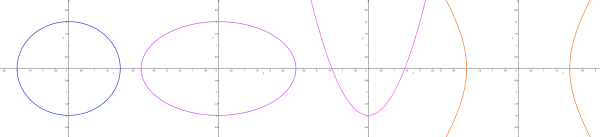
\includegraphics[width=1.0\linewidth]{pictures/kuzelosecky1.png}
    \caption*{Kuželosečky v rovině: kružnice, elipsa, parabola, hyperbola}
\end{figure}

\begin{figure}[h] 
    \centering    
    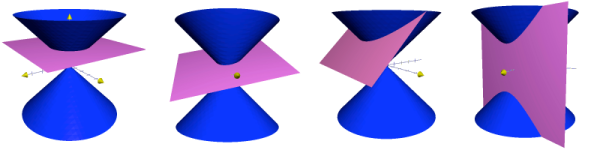
\includegraphics[width=1.0\linewidth]{pictures/kuzelosecky2.png}
    \caption*{Kuželosečky jako řezy kuželové plochy: kružnice, elipsa, parabola, hyperbola}
\end{figure}

Singulární kuželosečky, někdy se jim říká degenerované, vznikají, když rovina prochází vrcholem kuželů
nebo je rovnoběžná s pláštěm válce. Pokud jediným místem, kterým rovina prochází je právě vrchol
kuželů, namísto kružnice nebo elipsy dostáváme jediný bod. Pokud by rovina procházela vrchol kuželů
pod stejným úhlem jako je naklonění pláště kuželu, dostáváme dvojnásobnou přímku. Pokud prochází
rovina jak vrcholy kuželů i samotnými kuželi, získáváme dvě různoběžky, které se protínají právě
ve vrcholech kuželů.

Pro pochopení singulárních kuželoseček je nejlepší se podívat na simulace. Doporučuji 
například \href{https://www.intmath.com/plane-analytic-geometry/conic-sections-summary-
interactive.php}{odkaz}

\subsection*{Kružnice}
Kružnice je mnotina všech bodů v rovině, které mají od bodu $S$ stejnou vzdálenost $r$. Bod $S$ se 
nazává střed kružnice, hodnota $r$ se nazývá poloměr kružnice. Rovnice $(x = m)^2 + (y - n)^2 = r^2$
se nazývá středovou rovnicí kružnice se středem $S[m, n]$ a poloměrem $r$. Tato rovnice využíva
pythagorovou větu. Pokud by střed kružnice ležel v počátku, rovnice nabývá tvaru $x^2 + y^2 = r^2$.
Rovnice $x^2 + y^2 - 2mx - 2ny + p + m^2 + n^2 - r^2 = 0$. Tato rovnice vniká
roznásobením středové rovnice a nazývá se obecná rovnice. Z obecné rovnice se dělá středová rovnice
pomocí doplnění na čverec.

pozn. dodej ukazku doplneni na ctverec

Další úloha, kterou je rovnice tečny kružnice.

pozn. tohle proste dodelej

\subsection*{Elipsa}
\end{document}
